\documentclass[11pt]{article}
\usepackage[a4paper,margin=2.3cm]{geometry}
\usepackage[T1]{fontenc}
\usepackage{amsmath,amssymb,graphicx,booktabs,multirow,xcolor}
\usepackage[hidelinks]{hyperref}
\usepackage{caption,float}
\captionsetup{font=small,labelfont=bf}
\newcommand{\pending}{\textcolor{orange}{[pending]}}
\graphicspath{{figures/}}
\title{One Model, Any Camera --- Results Report\\[2pt]\large Advanced Computer Vision semester project}
\author{Shahnawaz Qureshi\\Sukkur IBA University}
\date{\today}
\begin{document}
\maketitle

\noindent\textbf{Project in one sentence.} We train a plant model once on hyperspectral images (204 bands) and use it,
without retraining and without any data from the new camera, on cheaper cameras (phone, drone, satellite), using
\emph{Stochastic Virtual Camera Training} (SVCT): every training batch is seen through a new random virtual camera.
The companion paper draft (\texttt{main.pdf}) gives the full method and discussion; this report lists every experiment
step by step with all numbers. All numbers are generated from the result files in the GitHub repository
(\url{https://github.com/ShahnawazQ007/one-model-many-camera}, folder \texttt{results/}).

\section*{Summary of findings}
\begin{enumerate}
\item \textbf{The problem is real.} A good 204-band model (0.821 cultivar accuracy) drops to 0.522 on seven unseen camera
profiles, and its fertilizer, grain-weight and $\Phi_{PSII}$ predictions become worse than guessing the mean
(negative $R^2$).
\item \textbf{The information is there.} Models trained separately on each camera reach 0.757 / fertilizer $R^2$ 0.765:
a few bands are enough; the 204-band model simply cannot use them.
\item \textbf{One SVCT model closes most of the gap} without data from the new cameras: 90\% of the cultivar gap
(interpolation variant, 0.732) and 84\% of the fertilizer gap (wavelength-stem variant, $R^2$ 0.582); robust to band
drift and calibration errors.
\item \textbf{Real second camera (fruit).} Trained only on the Specim FX10, SVCT predicts sugar content on the real Corning
camera as well as a model trained on Corning labels ($R^2$ 0.794 vs.\ 0.793).
\item \textbf{Real drone camera (leaves).} SVCT beats the plain model on all tasks, but a large gap to a model trained on
real drone labels remains, caused by the uncalibrated drone images.
\item \textbf{Costs and open points.} SVCT is weaker than the specialised model on the original 204-band camera;
consistency losses hurt; cross-validation (Step 9) is still running.
\end{enumerate}

\section{Data and splits (Step 3)}
\begin{itemize}
\item \textbf{HyperLeaf2024}: 2,410 wheat leaves, 204 bands, 36 field plots (4 cultivars $\times$ 3 fertilizer levels
$\times$ 3 plots). Targets: cultivar, grain weight, $g_{sw}$, $\Phi_{PSII}$, fertilizer. Official split (train and test
plots never shared) + plot-grouped 5-fold cross-validation.
\item \textbf{DeepHS Fruit v2}: 110 fruits (kaki, mango, papaya), each recorded by two real cameras (Specim FX10, 224 bands;
Corning microHSI 410, 249 bands). Split by fruit (the original lists share fruits = leakage).
\item \textbf{Estrada leaves}: 319 leaves (avocado, olive, grape) $\times$ 5 drying stages; ASD spectrometer + real
MicaSense images. Split by leaf.
\end{itemize}

\section{Is the camera simulator realistic? (Step 4)}
Simulating the same cheap cameras from the two real DeepHS cameras gives almost identical band values
(Pearson $r$ 0.94 blue, 0.991--0.998 other bands); the remaining difference is a per-band gain (0.86--1.35), so the
training calibration-gain range was widened to 0.8--1.25. The MicaSense images of the Estrada dataset are uncalibrated
digital numbers, so they cannot be used as an absolute check (band agreement $R^2$ 0.01--0.61).

\section{Held-out cameras}
\begin{table}[H]\centering\small
\caption{The seven camera profiles used only for testing.}
\begin{tabular}{@{}llcp{7.2cm}@{}}
\toprule
Camera & Type & Bands & Centre/FWHM (nm) \\
\midrule
Phone RGB$^\dagger$ & RGB & 3 & \footnotesize 460/80, 540/80, 610/70 \\
RGB+NIR$^\dagger$ & RGB+NIR & 4 & \footnotesize 460/80, 540/80, 610/70, 850/50 \\
DJI P4 Multispectral & UAV & 5 & \footnotesize 450/32, 560/32, 650/32, 730/32, 840/52 \\
MicaSense RedEdge-MX & UAV & 5 & \footnotesize 475/32, 560/27, 668/16, 717/12, 842/57 \\
MicaSense, no red edge$^\ddagger$ & control & 4 & \footnotesize 475/32, 560/27, 668/16, 842/57 \\
Parrot Sequoia & UAV & 4 & \footnotesize 550/40, 660/40, 735/10, 790/40 \\
Sentinel-2A MSI (VNIR) & satellite & 10 & \footnotesize 442.7/20, 492.7/65, 559.8/35, 664.6/30, 704.1/14, 740.5/14, 782.8/19, 832.8/105, 864.7/21, 945.1/19 \\
\bottomrule
\end{tabular}

\end{table}

\section{Baseline on the original camera (Step 5)}
\begin{table}[H]\centering\small
\caption{204-band models, official split. The ResNet18 with $2\times$ input and strong augmentation is the reference.}
\begin{tabular}{@{}lcccccc@{}}
\toprule
 & \multicolumn{2}{c}{Cultivar} & \multicolumn{4}{c}{$R^2$} \\
\cmidrule(lr){2-3}\cmidrule(l){4-7}
Model & Acc. & F1 & Grain & $g_{sw}$ & $\Phi_{PSII}$ & Fert. \\
\midrule
ResNet18, 204 bands & 0.730 & 0.705 & 0.712 & 0.114 & 0.407 & 0.774 \\
ResNet18, $2\times$ input, strong aug.\ (reference) & 0.821 & 0.805 & 0.584 & 0.077 & 0.524 & 0.759 \\
ConvNeXt-T, $2\times$ input, strong aug. & 0.768 & 0.764 & 0.714 & 0.037 & 0.471 & 0.785 \\
\bottomrule
\end{tabular}

\end{table}
A first fold of plot-grouped cross-validation with the plain ResNet18 gave cultivar 0.592 and fertilizer $R^2$ 0.806,
showing that results vary between plot splits; this is why Step 9 repeats the main experiment over five folds.

\section{The camera gap (Step 6) and SVCT (Step 7)}
\begin{table}[H]\centering\small\setlength{\tabcolsep}{3.5pt}
\caption{Mean over the seven held-out cameras. ``One model per camera'' needs labelled data from each camera.}
\resizebox{\linewidth}{!}{\begin{tabular}{@{}lcccccccc@{}}
\toprule
 & \multicolumn{4}{c}{Ideal cameras} & \multicolumn{2}{c}{Drift + calib.\ error} & \multicolumn{2}{c}{Full 204 bands} \\
\cmidrule(lr){2-5}\cmidrule(lr){6-7}\cmidrule(l){8-9}
Method & Cult.\ acc. & Fert.\ $R^2$ & Grain $R^2$ & $\Phi_{PSII}$ $R^2$ & Cult. & Fert. & Cult. & Fert. \\
\midrule
204-band model, bands interpolated & 0.522 & $-$0.364 & $-$0.685 & $-$0.562 & 0.505 & $-$0.488 & 0.821 & 0.759 \\
SVCT + wavelength stem (ours) & 0.670 & \textbf{0.582} & \textbf{0.528} & \textbf{0.254} & 0.640 & 0.462 & 0.660 & 0.589 \\
SVCT + interpolation (ours) & \textbf{0.732} & 0.468 & 0.429 & 0.227 & 0.703 & 0.409 & 0.689 & 0.629 \\
One model per camera$^\ast$ & 0.757 & 0.765 & 0.694 & 0.427 & -- & -- & -- & -- \\
\midrule
\quad gap closed, wavelength stem & 63\% & 84\% & 88\% & 83\% & & & & \\
\quad gap closed, interpolation & 90\% & 74\% & 81\% & 80\% & & & & \\
\bottomrule
\end{tabular}
}
\end{table}

\begin{table}[H]\centering\small
\caption{Per camera (ideal conditions). Base = 204-band model; Stem / Interp = SVCT variants; Own = model trained on
that camera.}
\begin{tabular}{@{}lcccccccc@{}}
\toprule
 & \multicolumn{4}{c}{Cultivar accuracy} & \multicolumn{4}{c}{Fertilizer $R^2$} \\
\cmidrule(lr){2-5}\cmidrule(l){6-9}
Camera & Base & Stem & Interp & Own & Base & Stem & Interp & Own \\
\midrule
Phone RGB$^\dagger$ & 0.360 & 0.550 & 0.768 & 0.795 & 0.297 & 0.278 & 0.368 & 0.720 \\
RGB+NIR$^\dagger$ & 0.527 & 0.704 & 0.679 & 0.771 & $-$0.486 & 0.596 & 0.324 & 0.730 \\
DJI P4 Multispectral & 0.588 & 0.726 & 0.730 & 0.782 & 0.206 & 0.709 & 0.474 & 0.791 \\
MicaSense RedEdge-MX & 0.528 & 0.741 & 0.751 & 0.760 & $-$0.356 & 0.699 & 0.646 & 0.778 \\
MicaSense, no red edge$^\ddagger$ & 0.543 & 0.696 & 0.763 & 0.784 & $-$1.211 & 0.534 & 0.531 & 0.731 \\
Parrot Sequoia & 0.499 & 0.629 & 0.701 & 0.687 & $-$1.372 & 0.643 & 0.322 & 0.812 \\
Sentinel-2A MSI (VNIR) & 0.609 & 0.641 & 0.732 & 0.718 & 0.374 & 0.617 & 0.608 & 0.791 \\
\bottomrule
\end{tabular}

\end{table}

\begin{figure}[H]\centering
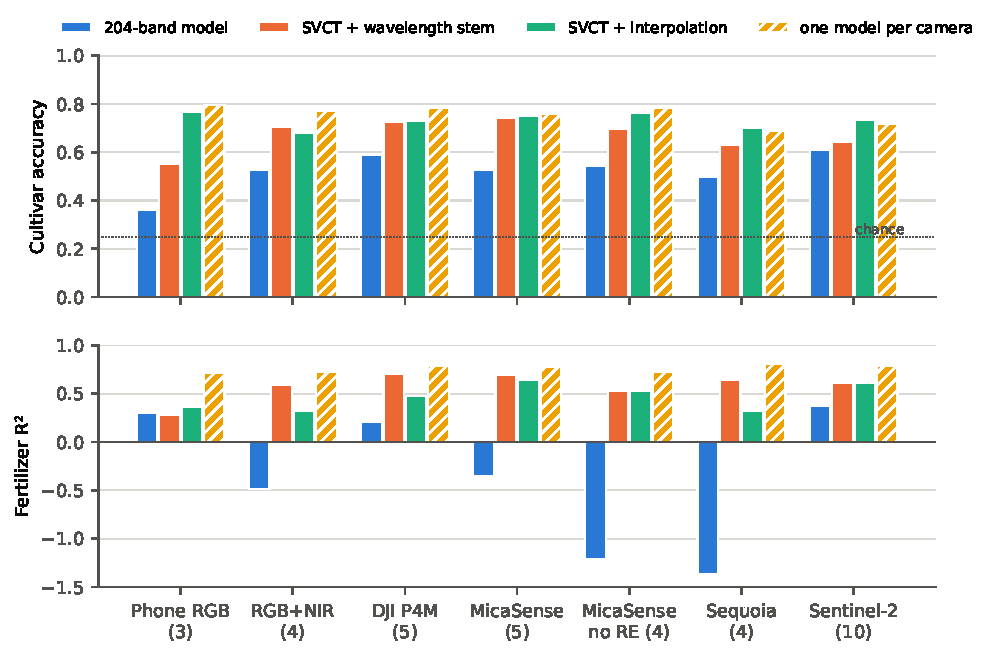
\includegraphics[width=\linewidth]{fig3_per_camera.pdf}
\caption{Per-camera results. Hatched: one model per camera.}
\end{figure}

\paragraph{Reading the results.} The phone is the hardest camera for the 204-band model (0.360, near chance); SVCT
with interpolation reaches 0.768 there, close to a phone-specific model (0.795). The two SVCT variants are complementary:
interpolation is better for cultivar, the wavelength stem for the physiological traits. On the full 204 bands SVCT is
lower than the specialised model (0.660--0.689 vs.\ 0.821), so in practice both models would be kept.

\section{Development rounds (ablation)}
\begin{table}[H]\centering\scriptsize\setlength{\tabcolsep}{3pt}
\caption{Three development rounds, same held-out cameras. The method was frozen after round 3.}
\begin{tabular}{@{}clcccccc@{}}
\toprule
 & & \multicolumn{4}{c}{7 held-out cameras (ideal)} & \multicolumn{2}{c}{204 bands} \\
\cmidrule(lr){3-6}\cmidrule(l){7-8}
Round & Variant & Cult. & Fert. & Grain & $\Phi_{PSII}$ & Cult. & Fert. \\
\midrule
1 & two views + symmetric consistency (w=1), uniform sampler & 0.502 & 0.480 & 0.464 & 0.203 & 0.562 & 0.543 \\
1 & same, without consistency & 0.639 & 0.456 & 0.356 & 0.285 & 0.707 & 0.609 \\
1 & same as first, interpolation instead of stem & 0.556 & 0.377 & 0.366 & 0.238 & 0.572 & 0.594 \\
2 & teacher distillation (w=0.5), structured sampler & 0.551 & 0.526 & 0.508 & 0.226 & 0.709 & 0.392 \\
2 & structured sampler, no consistency & 0.664 & 0.527 & 0.455 & 0.322 & 0.701 & 0.608 \\
2 & teacher distillation, interpolation & 0.647 & 0.418 & 0.387 & 0.234 & 0.645 & 0.681 \\
3 & final: no consistency, $p_{full}$=0.3, phone-weighted sampler, 150 ep. & 0.670 & 0.582 & 0.528 & 0.254 & 0.660 & 0.589 \\
3 & final, interpolation instead of stem & 0.732 & 0.468 & 0.429 & 0.227 & 0.689 & 0.629 \\
\bottomrule
\end{tabular}

\end{table}
Consistency losses (making two camera views of one leaf agree) lowered cultivar accuracy in both rounds where they were
tried, so they were removed. A sampler that practises RGB-like and multispectral layouts, more full-band batches and
longer training improved both variants.

\section{Cross-validation (Step 9)}
\begin{table}[H]\centering\small\setlength{\tabcolsep}{4pt}
\caption{Plot-grouped 5-fold cross-validation, mean $\pm$ s.d.\ over folds (mean over the seven held-out cameras).}
% Step 9 still running: placeholders
\begin{tabular}{@{}lccccc@{}}
\toprule
 & \multicolumn{3}{c}{Ideal cameras} & \multicolumn{2}{c}{Drift + calib.\ error} \\
\cmidrule(lr){2-4}\cmidrule(l){5-6}
Method & Cult.\ acc. & Fert.\ $R^2$ & Grain $R^2$ & Cult. & Fert. \\
\midrule
204-band model, bands interpolated & \pending & \pending & \pending & \pending & \pending \\
SVCT + wavelength stem (ours) & \pending & \pending & \pending & \pending & \pending \\
SVCT + interpolation (ours) & \pending & \pending & \pending & \pending & \pending \\
\bottomrule
\end{tabular}

\end{table}
\noindent\textcolor{orange}{Running on Kaggle at the time of writing (two notebooks, folds 0--2 and 3--4); the table will be
filled in automatically from the run outputs.}

\section{Real second cameras (Step 8)}
\begin{table}[H]\centering\scriptsize\setlength{\tabcolsep}{4pt}
\caption{DeepHS fruit: trained on FX10, tested on unseen fruits (5 folds $\times$ 3 seeds).}
\begin{tabular}{@{}lcccc@{}}
\toprule
Model & Fruit acc. & Ripeness acc. & Sugar $R^2$ & log-firmness $R^2$ \\
\midrule
\multicolumn{5}{@{}l}{\textit{Same camera (FX10)}} \\
\quad Plain MLP (FX10 only) & 0.982 $\pm$ 0.021 & 0.630 $\pm$ 0.103 & 0.773 $\pm$ 0.115 & 0.584 $\pm$ 0.230 \\
\quad SVCT, interpolation (FX10 only) & 0.979 $\pm$ 0.018 & 0.583 $\pm$ 0.048 & 0.799 $\pm$ 0.074 & 0.552 $\pm$ 0.186 \\
\quad SVCT, wavelength tokens (FX10 only) & 0.983 $\pm$ 0.025 & 0.589 $\pm$ 0.057 & 0.766 $\pm$ 0.081 & 0.568 $\pm$ 0.218 \\
\multicolumn{5}{@{}l}{\textit{Real Corning camera}} \\
\quad Plain MLP (FX10 only) & 0.838 $\pm$ 0.110 & 0.558 $\pm$ 0.051 & 0.547 $\pm$ 0.293 & $-$0.364 $\pm$ 0.623 \\
\quad SVCT, interpolation (FX10 only) & 0.971 $\pm$ 0.034 & 0.576 $\pm$ 0.036 & 0.794 $\pm$ 0.065 & 0.463 $\pm$ 0.244 \\
\quad SVCT, wavelength tokens (FX10 only) & 0.961 $\pm$ 0.051 & 0.589 $\pm$ 0.068 & 0.731 $\pm$ 0.123 & 0.455 $\pm$ 0.341 \\
\quad Trained on Corning labels$^\ast$ & 0.995 $\pm$ 0.009 & 0.580 $\pm$ 0.095 & 0.793 $\pm$ 0.092 & 0.566 $\pm$ 0.251 \\
\multicolumn{5}{@{}l}{\textit{Real Corning, reduced to the 7 camera profiles (mean)}} \\
\quad Plain MLP (FX10 only) & 0.531 $\pm$ 0.117 & 0.444 $\pm$ 0.080 & 0.014 $\pm$ 0.459 & $-$3.858 $\pm$ 2.847 \\
\quad SVCT, interpolation (FX10 only) & 0.934 $\pm$ 0.033 & 0.543 $\pm$ 0.041 & 0.651 $\pm$ 0.078 & 0.403 $\pm$ 0.155 \\
\quad SVCT, wavelength tokens (FX10 only) & 0.945 $\pm$ 0.023 & 0.574 $\pm$ 0.052 & 0.648 $\pm$ 0.120 & 0.376 $\pm$ 0.320 \\
\multicolumn{5}{@{}l}{\textit{FX10, reduced to the 7 camera profiles (mean)}} \\
\quad Plain MLP (FX10 only) & 0.716 $\pm$ 0.095 & 0.412 $\pm$ 0.082 & 0.098 $\pm$ 0.327 & $-$2.742 $\pm$ 2.134 \\
\quad SVCT, interpolation (FX10 only) & 0.947 $\pm$ 0.024 & 0.550 $\pm$ 0.036 & 0.697 $\pm$ 0.087 & 0.459 $\pm$ 0.152 \\
\quad SVCT, wavelength tokens (FX10 only) & 0.960 $\pm$ 0.028 & 0.573 $\pm$ 0.045 & 0.705 $\pm$ 0.096 & 0.469 $\pm$ 0.239 \\
\bottomrule
\end{tabular}

\end{table}
\begin{table}[H]\centering\scriptsize\setlength{\tabcolsep}{4pt}
\caption{Estrada leaves: trained on the spectrometer, tested on unseen leaves (5 folds $\times$ 3 seeds).}
\begin{tabular}{@{}lcccc@{}}
\toprule
Model & Crop acc. & Stage acc. & Chlorophyll $R^2$ & Water (FMC) $R^2$ \\
\midrule
\multicolumn{5}{@{}l}{\textit{Same sensor (spectrometer, 400--1000 nm)}} \\
\quad Plain MLP (spectrometer only) & 0.980 $\pm$ 0.007 & 0.899 $\pm$ 0.017 & 0.860 $\pm$ 0.023 & 0.934 $\pm$ 0.009 \\
\quad SVCT, interpolation & 0.924 $\pm$ 0.013 & 0.681 $\pm$ 0.020 & 0.812 $\pm$ 0.024 & 0.750 $\pm$ 0.020 \\
\quad SVCT, wavelength tokens & 0.912 $\pm$ 0.016 & 0.647 $\pm$ 0.022 & 0.798 $\pm$ 0.029 & 0.708 $\pm$ 0.019 \\
\multicolumn{5}{@{}l}{\textit{Real MicaSense camera}} \\
\quad Plain MLP (spectrometer only) & 0.457 $\pm$ 0.044 & 0.198 $\pm$ 0.028 & $-$0.002 $\pm$ 0.243 & $-$0.154 $\pm$ 0.114 \\
\quad SVCT, interpolation & 0.524 $\pm$ 0.031 & 0.275 $\pm$ 0.016 & 0.465 $\pm$ 0.056 & 0.149 $\pm$ 0.086 \\
\quad SVCT, wavelength tokens & 0.543 $\pm$ 0.035 & 0.271 $\pm$ 0.017 & 0.425 $\pm$ 0.041 & 0.192 $\pm$ 0.046 \\
\quad Trained on simulated MicaSense$^\S$ & 0.593 $\pm$ 0.051 & 0.270 $\pm$ 0.018 & 0.356 $\pm$ 0.076 & $-$0.115 $\pm$ 0.110 \\
\quad Trained on real MicaSense labels$^\ast$ & 0.927 $\pm$ 0.009 & 0.525 $\pm$ 0.028 & 0.800 $\pm$ 0.017 & 0.514 $\pm$ 0.033 \\
\multicolumn{5}{@{}l}{\textit{Simulated, 7 camera profiles (mean)}} \\
\quad Plain MLP (spectrometer only) & 0.522 $\pm$ 0.026 & 0.176 $\pm$ 0.014 & $-$0.366 $\pm$ 0.371 & $-$0.633 $\pm$ 0.141 \\
\quad SVCT, interpolation & 0.810 $\pm$ 0.017 & 0.515 $\pm$ 0.016 & 0.721 $\pm$ 0.027 & 0.539 $\pm$ 0.026 \\
\quad SVCT, wavelength tokens & 0.843 $\pm$ 0.017 & 0.539 $\pm$ 0.020 & 0.733 $\pm$ 0.027 & 0.564 $\pm$ 0.026 \\
\bottomrule
\end{tabular}

\end{table}
\begin{figure}[H]\centering
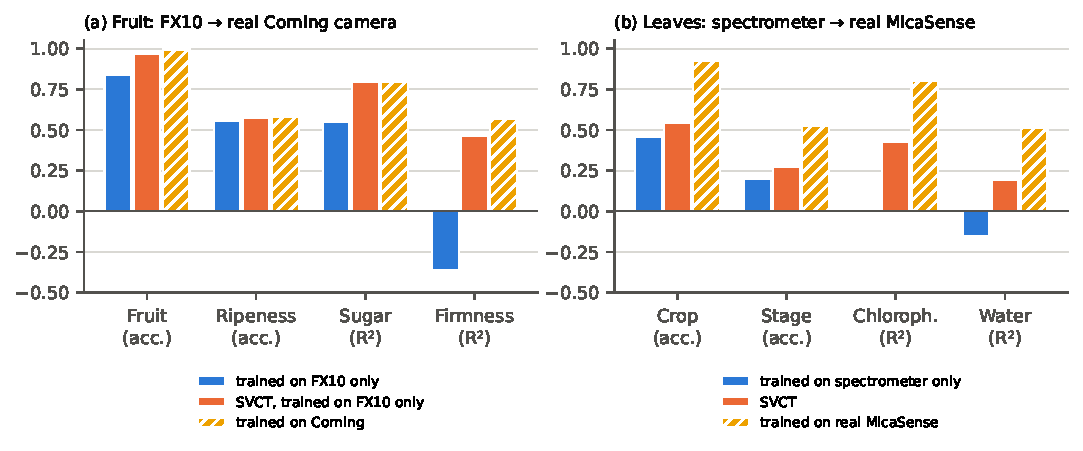
\includegraphics[width=\linewidth]{fig4_real_cameras.pdf}
\caption{Real second cameras. Hatched: trained on labelled data of the target camera.}
\end{figure}

\paragraph{Reading the results.} On fruit, SVCT matches the Corning-trained model for sugar without any Corning labels
and fixes the negative firmness score of the plain model. Ripeness stays around 0.58 for every model, including the
Corning-trained one, so it is a label/data limit. On leaves, the real drone camera remains difficult for all
simulation-trained models (even one trained on simulated MicaSense bands reaches only 0.593 crop accuracy), because the
released drone images are not radiometrically calibrated.

\section{Limitations and next steps}
\begin{itemize}
\item Finish Step 9 (cross-validation) and add paired statistical tests.
\item Compare with published camera-agnostic methods (Hyve, CARL).
\item Replace the approximate phone and RGB+NIR responses with measured ones.
\item Field drone data with reflectance panels for a calibrated real-camera test.
\item Product: package + demo app (``AnyCam'') that takes a camera's band list and returns predictions.
\end{itemize}

\end{document}
